\documentclass[11pt]{beamer}
%\documentclass[11pt,handout]{beamer}

%%% PACKAGES
\usepackage[utf8]{inputenc}  % italian symbols.
\usepackage[T1]{fontenc}     % define T1 charset for out files.
\usepackage[italian]{babel}  % italian latex typo conventions.
\usepackage{csquotes}        % needed by babel.
\usepackage{amsmath}         % math features.
\usepackage{amsthm}          % math theorems.
\usepackage{amssymb}         % math symbols.
\usepackage{graphicx}        % images managing.
\usepackage{booktabs}        % \toprule, \midrule and \bottomrule in tables.
\usepackage{algorithm}       % algorithm block.
\usepackage{algcompatible}
\usepackage{algpseudocode}   % style for (autoimported) package algorithmicx.
\usepackage{csquotes}        % smart quotes.
\usepackage[
backend=biber,
style=numeric,
citestyle=numeric  % numeric, alphabetic
]{biblatex}                  % bib management. %bibtex

%%% MODE
\mode<presentation> {

    % THEME

    %\usetheme{default}
    %\usetheme{AnnArbor}
    %\usetheme{Antibes}
    %\usetheme{Bergen}        % commented left
    %\usetheme{Berkeley}      % menu left
    %\usetheme{Berlin}
    %\usetheme{Boadilla}      % nice, no top menu
    %\usetheme{CambridgeUS}   % nice menu and footer
    %\usetheme{Copenhagen}
    %\usetheme{Darmstadt}
    %\usetheme{Dresden}
    %\usetheme{Frankfurt}     % top bullets, no info below
    %\usetheme{Goettingen}    % no
    %\usetheme{Hannover}      % no
    %\usetheme{Ilmenau}       % not bad: bullets, sections, ... but too many rows
    %\usetheme{JuanLesPins}   % tree menu
    %\usetheme{Luebeck}       % very nice menu
    %\usetheme{Madrid}        % default
    %\usetheme{Malmoe}
    %\usetheme{Marburg}
    %\usetheme{Montpellier}
    %\usetheme{PaloAlto}
    %\usetheme{Pittsburgh}    % clean
    %\usetheme{Rochester}
    %\usetheme{Singapore}     % not bad, no info below
    %\usetheme{Szeged}
    %\usetheme{Warsaw}
    \usetheme[nologos]{Padova}  % University of Pauda.

    % COLOR THEME

    %\usecolortheme{albatross}     % horrible
    %\usecolortheme{beaver}        % red blue
    %\usecolortheme{beetle}        % horrible
    %\usecolortheme{crane}         % nice: yellow, orange
    %\usecolortheme{dolphin}       % simil default
    %\usecolortheme{dove}          % black and white
    %\usecolortheme{fly}           % horrible
    %\usecolortheme{lily}          % nice, clean blue
    %\usecolortheme{orchid}        % like default
    %\usecolortheme{rose}          % like default, very good
    %\usecolortheme{seagull}       % grey
    %\usecolortheme{seahorse}      % light lavanda
    %\usecolortheme{whale}         % like default
    %\usecolortheme{wolverine}     % yello blue

    \usefonttheme{professionalfonts}

    % To remove the footer line in all slides uncomment this line
    %\setbeamertemplate{footline}

    % To replace the footer line in all slides with a simple slide
    % count uncomment this line
    %\setbeamertemplate{footline}[page number]

    % To remove the navigation symbols from the bottom of all
    % slides uncomment this line
    %\setbeamertemplate{navigation symbols}{}

    % blocks
    %\setbeamertemplate{blocks}[rounded][shadow=true]

} % /mode<presentation>

% top menu
%\useoutertheme[subsection=false]{miniframes}

%\setbeamercolor{block title}{use=structure,fg=white,bg=blue!75!black}
%\setbeamercolor{block body}{use=structure,fg=black,bg=white!20!white}

% step by step
%\setbeamercovered{transparent}

%%% CONFIGURATIONS
%% Special letters denoting sets and algebras.
\providecommand*{\Nset}{\mathbb{N}}             % Naturals
\providecommand*{\Qset}{\mathbb{Q}}             % Rationals
\providecommand*{\Zset}{\mathbb{Z}}             % Integers
\providecommand*{\Rset}{\mathbb{R}}             % Reals

%% Calligraphic alphabet.
\newcommand*{\calA}{\ensuremath{\mathcal{A}}}
\newcommand*{\calB}{\ensuremath{\mathcal{B}}}
\newcommand*{\calC}{\ensuremath{\mathcal{C}}}
\newcommand*{\calD}{\ensuremath{\mathcal{D}}}
\newcommand*{\calE}{\ensuremath{\mathcal{E}}}
\newcommand*{\calF}{\ensuremath{\mathcal{F}}}
\newcommand*{\calG}{\ensuremath{\mathcal{G}}}
\newcommand*{\calH}{\ensuremath{\mathcal{H}}}
\newcommand*{\calI}{\ensuremath{\mathcal{I}}}
\newcommand*{\calJ}{\ensuremath{\mathcal{J}}}
\newcommand*{\calK}{\ensuremath{\mathcal{K}}}
\newcommand*{\calL}{\ensuremath{\mathcal{L}}}
\newcommand*{\calM}{\ensuremath{\mathcal{M}}}
\newcommand*{\calN}{\ensuremath{\mathcal{N}}}
\newcommand*{\calO}{\ensuremath{\mathcal{O}}}
\newcommand*{\calP}{\ensuremath{\mathcal{P}}}
\newcommand*{\calQ}{\ensuremath{\mathcal{Q}}}
\newcommand*{\calR}{\ensuremath{\mathcal{R}}}
\newcommand*{\calS}{\ensuremath{\mathcal{S}}}
\newcommand*{\calT}{\ensuremath{\mathcal{T}}}
\newcommand*{\calU}{\ensuremath{\mathcal{U}}}
\newcommand*{\calV}{\ensuremath{\mathcal{V}}}
\newcommand*{\calW}{\ensuremath{\mathcal{W}}}
\newcommand*{\calX}{\ensuremath{\mathcal{X}}}
\newcommand*{\calY}{\ensuremath{\mathcal{Y}}}
\newcommand*{\calZ}{\ensuremath{\mathcal{Z}}}

% **********************************************************
% Luca Parolari <luca.parolari23@gmail.com>
% -- macros for bachelor thesis <TITLE> <url_here>

\newcommand*{\clpset}{CLP(\calS\calE\calT)}                % CLP(SET)
\newcommand*{\satset}{SAT\textsubscript{\calS\calE\calT}}  % SAT_SET
\newcommand*{\calset}{\calS\calE\calT}                     % SET
\newcommand*{\satbr}{SAT\textsubscript{\calB\calR}}        % SAT_BR
\newcommand*{\lbr}{\textit{L}\textsubscript{BR}}           % L_BR
\newcommand*{\lset}{\textit{L}\textsubscript{\calS\calE\calT}} % L_SET
\newcommand*{\setlog}{$\{$log$\}$}                         % {log}
\newcommand*{\jsetl}{JSetL}                                 % JSetL

% Dotted letters
\newcommand*{\dotA}{\ensuremath{\dot{A}}}
\newcommand*{\dotB}{\ensuremath{\dot{B}}}
\newcommand*{\dotC}{\ensuremath{\dot{C}}}
\newcommand*{\dotx}{\ensuremath{\dot{x}}}

\newcommand*{\fixme}[1]{\footnote{\textbf{FIXME:} {#1}}}
\newcommand*{\todo}[1]{\footnote{\textbf{TODO:} {#1}}}




%-------------------------------------------------------------------
%   TITLE PAGE
%-------------------------------------------------------------------

% The short title appears at the bottom of every slide,
% the full title is only on the title page
\title[Introduzione]{Introduzione all'informatica}
\subtitle{Cos'è l'informatica?}
\author{Luca Parolari}
\date{08 novembre 2019}

\begin{document}

    \begin{frame}[plain]
        \maketitle
    \end{frame}

    \section{Introduzione}

    \begin{frame}
        \frametitle{Cos'è l'informatica}

        \centering
        Quiz: \href{https://pollev.com/lucaparolari783}{https://pollev.com/lucaparolari783}
    \end{frame}

    \begin{frame}
        \frametitle{Cos'è l'informatica?}

        \blockquote{Computer Science is no more about computers than astronomy is about telescopes.}

        \begin{flushright}
            Senza fonte: Edsger Wybe Dijkstra\\
            (Rotterdam 1930 - Nuenen 2002)
        \end{flushright}
    \end{frame}

    \begin{frame}
        \frametitle{Cos'è l'informatica?}

        \blockquote{Computer science is the study of algorithms,    including their formal and mathematical properties, their hardware realizations, their linguistic realizations and their application.}

        \begin{flushright}
            N.E. Gibbs, A.B.Tucker,\\ ``A model curriculum for a liberal arts degree in CS'',\\ Communications of ACM 29(3), 1986
        \end{flushright}
    \end{frame}

    \begin{frame}
        \frametitle{Cos'è l'informatica?}

        L'informatica è la scienza che si occupa del trattamento dell'informazione mediante \alert{procedure automatizzate}. In particolare ha per oggetto lo studio dei fondamenti teorici dell'informazione, della sua computazione a livello logico e delle tecniche pratiche per la sua implementazione e applicazione in sistemi elettronici automatizzati detti quindi sistemi informatici. (Wikipedia)
    \end{frame}

    \begin{frame}
        \frametitle{Un po' di storia}
        \framesubtitle{Antichità}

        \begin{columns}
            \column{0.5\textwidth}

            Le radici sono antichissime!

            \begin{itemize}
                \item \textbf{L'abaco}, uno dei più antichi strumenti di computazione.

                \item \textbf{La macchina di Antikythera}, il più antico calcolatore meccanico conosciuto.
            \end{itemize}

            \column{0.5\textwidth}
            \begin{figure}
                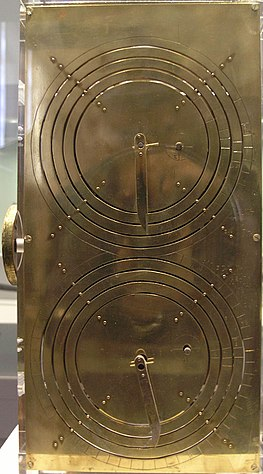
\includegraphics[scale=0.3]{img/macchina-antikythera.jpg}
                \caption{Ricostruzione della macchina di Antikythera}
            \end{figure}
        \end{columns}
    \end{frame}

    \begin{frame}
        \frametitle{Un po' di storia}
        \framesubtitle{XVII, XVIII e XIX secolo}

        \begin{columns}
            \column{0.55\textwidth}
            \begin{itemize}
                \item Gottfried Wilhelm \textbf{Leibniz} sviluppa la logica come disciplina matematica e formale, con i suoi scritti sul \alert{sistema numerico binario} (1702).

                \item George \textbf{Boole} crea un sistema nel quale è possibile trattare ogni relazione logica attraverso l'utilizzo di \alert{formule algebriche} (1854).
            \end{itemize}

            \column{0.45\textwidth}
            \begin{figure}
                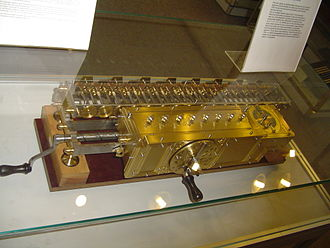
\includegraphics[scale=0.4]{img/calcolatrice-leibniz.jpg}
                \caption{Calcolatrice di Leibniz}
            \end{figure}
        \end{columns}
    \end{frame}

    \begin{frame}
        \frametitle{Un po' di storia}
        \framesubtitle{XX secolo}

        \begin{itemize}
            \item Alan \textbf{Turing} riesce nell'impresa di decifrare i messaggi in codice utilizzati dai tedeschi con la macchina Enigma. Fornisce importanti contributi nel campo della \alert{computabilità}.

            \item Kurt \textbf{Gödel}, dà un'enorme spinta alla teoria informatica di base e ai sistemi formali che la sorreggono come le \alert{funzioni ricorsive}, il \alert{lambda calcolo} e la \alert{macchina di Turing}.
        \end{itemize}
    \end{frame}

    \begin{frame}
        \frametitle{Un lato oscuro}
        \framesubtitle{Il razzo Ariane 5}

        \centering
        Quiz: \href{https://www.kahoot.it}{https://www.kahoot.it}

        \begin{figure}
            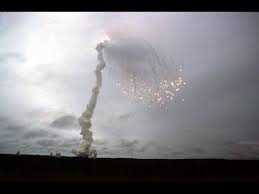
\includegraphics[scale=0.7]{img/ariane-5-explosion.jpg}
            \caption{Razzo Ariane 5}
        \end{figure}
    \end{frame}

    \begin{frame}
        \frametitle{Gli ultimi anni}

        Due sono stati i grossi ``boost'' per l'informatica:

        \begin{itemize}
            \item \textbf{internet}, che ha aumentato esponenzialmente l'interscambio di informazioni;
            \item la \textbf{potenza} dei processori, che ha permesso di creare applicazioni sempre più complesse.
        \end{itemize}
    \end{frame}

    \begin{frame}
        \frametitle{Hardware}
        \framesubtitle{La macchina di von Neumann}

        \begin{figure}
            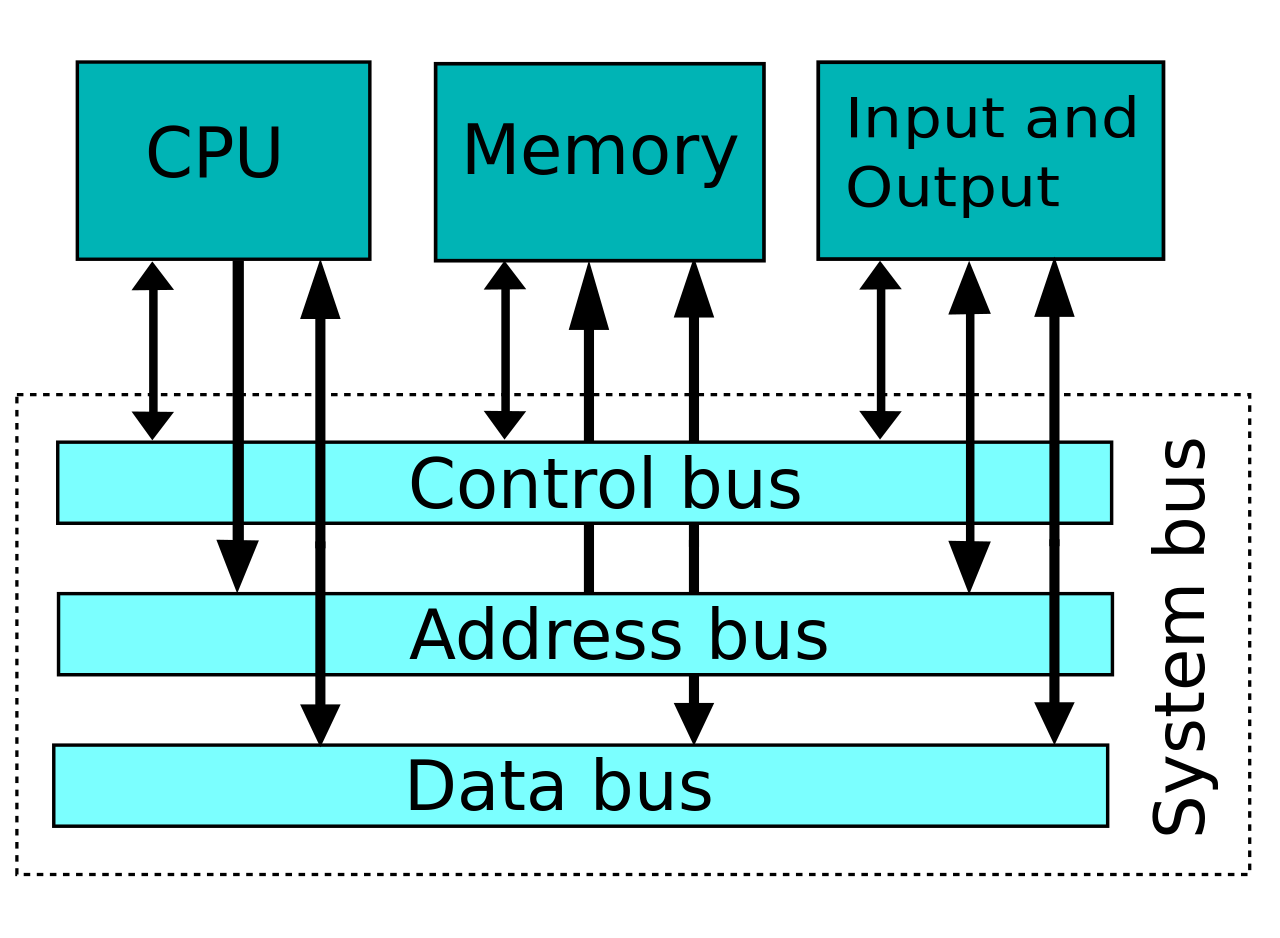
\includegraphics[scale=0.15]{img/macchina-von-neumann.png}
            \caption{Architettura di von Neumann}
        \end{figure}
    \end{frame}

    \begin{frame}
        \frametitle{Software}
        \framesubtitle{Classifica linguaggi di programmazione}

        \begin{figure}
            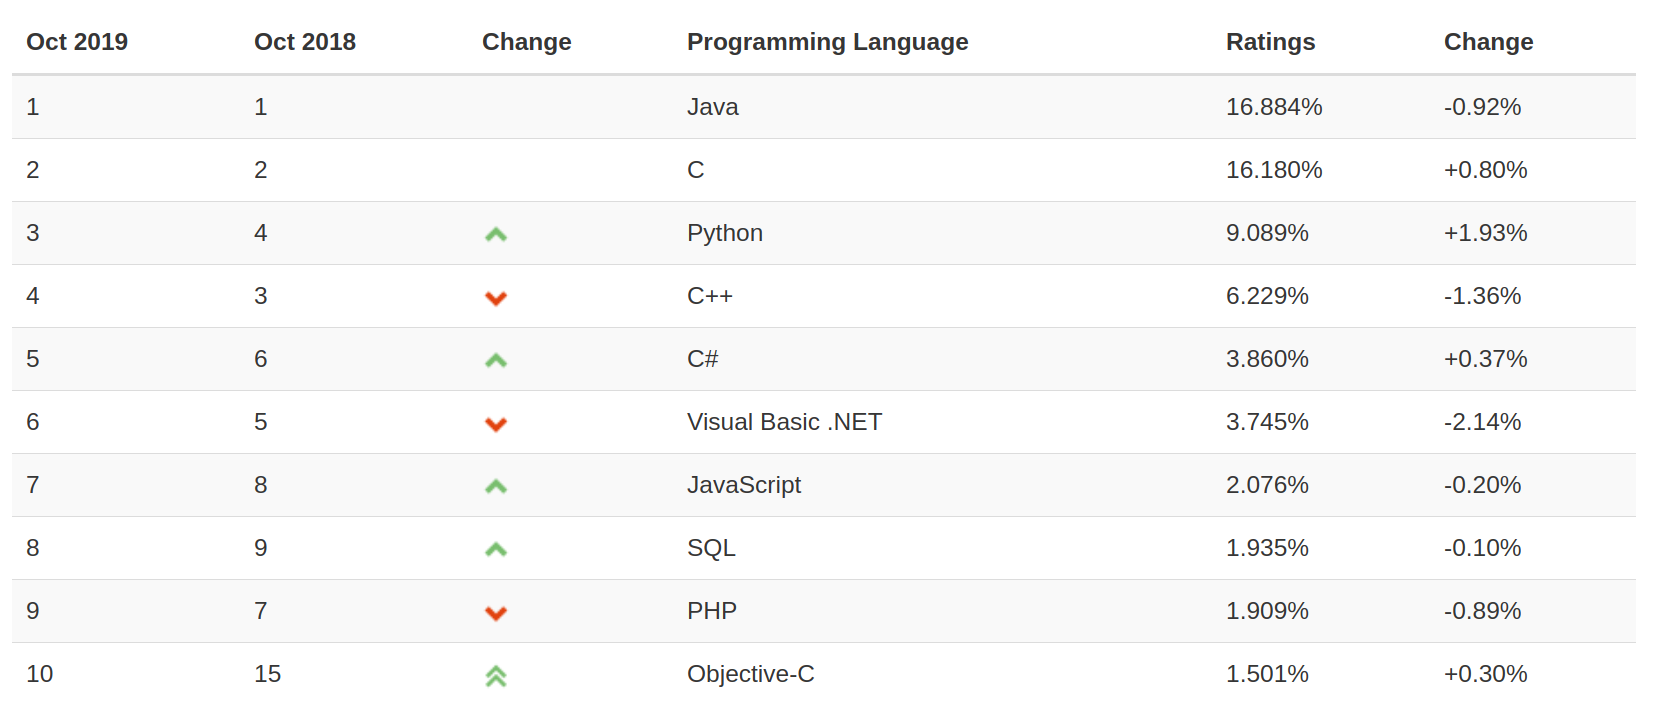
\includegraphics[scale=0.2]{img/classifica-lp-tiobe.png}
            \caption{Top 10 linguaggi di programmazione, indice TIOBE}
        \end{figure}
    \end{frame}

    \begin{frame}
        \frametitle{Risorse}

        \begin{itemize}
            \item P. Camagni e R. Nicolassy, Corso di informatica linguaggio C e C++ (Hoeply)
            \item Moodle oppure Google Classroom
        \end{itemize}
    \end{frame}

\end{document}